% Co-authored-by: cherusk <10729954+cherusk@users.noreply.github.com>
\documentclass[11pt,a4paper]{article}
\usepackage[utf8]{inputenc}
\usepackage[T1]{fontenc}
\usepackage{libertine}
\usepackage[libertine]{newtxmath}
\usepackage{amsmath}
\usepackage{graphicx}
\usepackage{xcolor}
\usepackage{booktabs}
\usepackage{subcaption}
\usepackage{titlesec}
\usepackage{hyperref}
\usepackage[margin=2.6cm]{geometry}

\title{From Edges to Curves: Calibration of Autonomous Coupling
       Characterization in Live Systems}
\author{
  Matthias Tafelmeier \\
  Independent Scientist \\
  Hof, Germany \\
  \href{https://orcid.org/0009-0005-7399-5584}{ORCID: 0009-0005-7399-5584}
}
\date{}

\begin{document}
\maketitle

\begin{abstract}
Autonomous agents that share a substrate couple through it, and
prior work established that such hidden coupling can be
\emph{detected} by guardrail-bounded probing between the agents
themselves. This paper asks the next question: how accurately can
that coupling be \emph{characterized} --- measured as a response
curve, with error bars, while the system is live? We describe the
characterization walk, a self-directed measurement procedure whose
sampling heuristic is disagreement-driven refinement and whose
stopping rule is denominated in units of measured ignorance, and we
calibrate it against closed-form planted truth across a 32-cell
grid: coupling strengths $0.0$ to $0.9$, Gaussian noise to
$\sigma{=}0.10$, four response shapes, six wiring topologies, and
two regimes of non-stationarity. Every certified point falls within
its own reported uncertainty (worst $1.76\sigma$); no sentinel ---
dead parameter, reverse direction, empty channel, zero coupling ---
produces structure; anchor and boundary cells repeat across seeds.
The certificate covers range, error, cost per curve, and the
conditions under which the walk correctly refuses to converge.
\end{abstract}

\noindent\textbf{Keywords:} active probing, autonomous agents,
multi-agent systems, coupling discovery, characterization walk,
response curve, calibration, uncertainty quantification, system
identification, design of experiments, live systems, complex systems

\section{Introduction}
\label{sec:intro}

When two autonomous agents tend the same substrate, each one's
parameter changes propagate into the other's objectives. The
coupling is real, hidden, and --- as prior work established
~\cite{p1} --- discoverable: a push/hold/pause protocol with
block-step detection recovers which pairs of agents are coupled,
without central observers and without disrupting the system. But
detection answers a binary question. It says nothing about
\emph{how much}, in what shape, or with what confidence --- and it
is exactly those quantities that any downstream use of the
discovered structure requires. Prediction needs the response
function, not the arrow. Steering needs the curve, not the scalar.

This paper closes that gap and calibrates what closes it. The
procedure is the \emph{characterization walk}
(\S\ref{sec:method}): the sending agent probes its parameter axis
at self-chosen levels while the receivers hold still; readings are
block medians carrying error bars from local noise; the walk stops
when its remaining ignorance is priced below what further trials
are worth. The question this paper answers is not whether the walk
works --- the campaign's design assumes no minimum performance bar
--- but \emph{where it works, how well, and at what cost}: a
calibration certificate, measured against planted truth that the
walking agents never see.

The contributions are the certificate's clauses:
\begin{enumerate}
\item \textbf{Accuracy.} Across 32 cells, every certified
measurement point falls within its own reported error bar --- worst
case $1.76\sigma$ against closed-form ground truth, median near
one bar-width (\S\ref{sec:results}).
\item \textbf{Envelope.} The working range is measured, not
asserted: coupling strength down to $0.1$ (below the detection
floor of~\cite{p1}), Gaussian noise to $\sigma{=}0.10$ --- including
the exact condition at which block-step detection fails,
characterized here at $0.62\sigma$ --- all four base response
shapes, and six wiring topologies (\S\ref{sec:floor}--\ref{sec:shapes}).
\item \textbf{Non-stationarity.} Under noise that grows through a
run, error bars fatten in real time and the truth stays inside
them; under drifting coupling strength the walk tracks the moving
edge; under fast drift it returns an honest non-convergence rather
than a fabricated average (\S\ref{sec:nonstat}).
\item \textbf{Cost.} Trials-to-retirement scales with signal, not
with schedule: the stopping rule is the procedure's own cost model
(\S\ref{sec:cost}).
\item \textbf{Specificity.} Zero invented structure across every
planted sentinel and a zero-coupling control; repeatability of
every verdict across seeds at the anchor and both boundary corners
(\S\ref{sec:repeat}).
\end{enumerate}

We report the boundary alongside the certificate
(\S\ref{sec:boundaries}): additive-linear coupling physics, a quiet
bench, a mathematical substrate class, multi-sender coverage
limits, and an initialization artifact --- each named as measured.
\S\ref{sec:honesty} states the measurement-honesty methodology
that the campaign enforced on itself, and \S\ref{sec:discussion}
discusses what a certified curve is the basis for. All tables and
figures regenerate from the retained evidence by a shipped script;
every run carries an external identifier.

\section{Method: The Characterization Walk}
\label{sec:method}

Detection, as established in prior work~\cite{p1}, answers a binary
question per pair of agents: does a coupling edge exist? The present
this paper's procedure answers the quantitative one: what does the response
\emph{look like}? We refer to the measurement procedure as the
\emph{characterization walk}. Its contract with the substrate is
unchanged from the detection protocol --- turn-taking under a
group-scoped lease, guardrail-bounded pushes, ABA block structure ---
so we describe here only what is new: how levels are chosen, how
uncertainty is carried, and when the walk stops.

\paragraph{Coverage walk.}
The sender does not grid its parameter axis. Starting from the axis
endpoints and midpoint, each subsequent probe level is placed inside
the \emph{gap} between adjacent measured points where the product of
observed jump and gap width is largest --- the region where an
unsampled response shape could hide the most structure. The receiver
listens from the first trial; its quiescence is what makes every
reading attributable to the sender's intervention rather than to its
own exploration.

\paragraph{Uncertainty-aware curves.}
Each level is held for a block of trials; the reading is the block
median, and its error bar is the median absolute deviation of the same
block. No model of the response is fitted at any point: the curve is
the set of (level, value, bar) triples, blended across repeat visits
by inverse-variance weighting. The bars are therefore measurements of
the substrate's noise, not statements of confidence in a fit.

\paragraph{Priced stop.}
When does the walk stop adding levels? The rule rests on a single
question, asked about every gap between two adjacent measured
points: \emph{how much response could still be hiding in there?}
Between two measurements, the curve could rise, dip, or jump ---
the two points do not constrain it. What bounds the possibility is
the pair of jumps at the gap's edges: a curve that changed sharply
on both sides of an unsampled region might change sharply inside
it, while a curve that is flat on both sides cannot hide much,
whatever its shape. The walk therefore prices each gap as
\begin{equation}
\text{ignorance}(g) \;=\; \frac{|\Delta y_{\text{adjacent}}| \times
\text{width}(g)}{\text{range}(y)} ,
\label{eq:ignorance}
\end{equation}
the response change that could plausibly hide between the two
measured points, expressed in units of the curve's own observed
range. A gap is \emph{resolved} when this price falls below the
local error bar: at that point, learning what lies inside the gap
would change the curve by less than the amount the measurements
themselves are uncertain by, so the trials cannot pay for
themselves.

The walk retires a curve under a two-key rule: the curve must be
converged (successive refinements changing it by less than a small
threshold) \emph{and} every remaining gap must be priced below its
local bar. Two examples fix the idea. In the weakest cell of the
campaign (strength $0.1$), the whole curve spans roughly three
error bars; after three well-placed levels, every unsampled gap
could hide at most a fraction of a bar, and the walk stops --- three
points are a complete measurement of a curve that small at that
noise. In the threshold cell, by contrast, the gaps flanking the
discontinuity keep their prices high no matter how often they are
split, because the adjacent jumps are large; the walk refines
fifteen levels and still retires with the cliff bracketed rather
than resolved, which is exactly the honest outcome: the jump is
localized to a narrow level interval, and nothing inside that
interval could have been measured more precisely than the bars
allow.

The rule makes walk depth a property of the substrate rather than
a configuration parameter: weak signals retire at few levels,
steep flanks attract refinement, and the walk never claims
resolution it declined to buy.

In short: a self-directed calibration method whose sampling
heuristic is disagreement-driven refinement and whose stopping rule
is denominated in units of measured ignorance.

\section{Experimental Design}
\label{sec:design}

\paragraph{The bench as oracle.}
All measurements run on a parameterizable substrate in which coupling
is planted and its ground truth is a closed-form formula. Each node
maps its parameters to two objectives through a selectable base
function --- linear $w\,x$, polynomial $w\,x^2$, threshold
$w\,\mathbb{1}[x>0.5]$, or saturation $w\,x/(1+4|x-0.5|)$ --- and each
directed edge feeds one channel of one node with the (noisy) channel
value of another, scaled by a planted strength. The planted response
of a cell is therefore
\begin{equation}
y^*(L) \;=\; s \cdot w \cdot \left( f(L/100) - f(0.5) \right),
\label{eq:truth}
\end{equation}
known to the scoring harness and invisible to the agents: the walkers
receive only noisy objective readings over an HTTP interface, never
the topology, the formula, or the strength. Scoring is thus fully
external: for every measured point we compute
$|y - y^*|/\sigma_{\text{bar}}$, the deviation in units of the
walk's own reported uncertainty.

\paragraph{The grid.}
Thirty-two cells span the axes of the claim. Coupling strength from
$0.0$ to $0.9$ at low noise traces the \emph{floor}; Gaussian noise
$\sigma$ from $0.02$ to $0.10$ at high strength traces the
\emph{wall}, including the exact condition ($0.5$ at $\sigma{=}0.10$)
at which block-step detection was reported to fail in prior
work~\cite{p1}. All four base functions are characterized at two
strengths. Six wiring topologies exercise routing and structure:
cross-channel (the edge feeds the second objective), bidirectional,
fan-in (two senders, one receiver), fan-out (one sender, two
receivers), a four-node diamond and a three-node chain --- the last
two banked as composition data for the successor question rather than
scored here. Non-stationarity enters twice: noise that grows through
the run, and edge strength that drifts upward through the run
(fast and slow rates). Finally, the anchor and both boundary corners
are repeated with a different random seed.

\paragraph{Sentinels.}
Every cell plants its own traps alongside the signal: dead parameters
(zero weight on the carrier channel) that must read flat, the reverse
direction that must read flat, an empty channel that must read flat,
and one zero-coupling cell in which \emph{nothing} may show
structure. These are the false-positive controls of the
characterization claim; throughout the campaign not one of them
produced a non-flat reading above noise.

\paragraph{Doctrine.}
The sweep is calibration, not pass/fail. No minimum performance bar is
imposed; expected degradation at the map's edge is reported as a
result, and only failures in the strong-signal/low-noise corner ---
the corner where the procedure contradicts itself --- would indicate
a defect. All runs execute the same engine build; the walker is
frozen for the campaign's duration. Every run's curves, per-point
bars, and external run identifiers are retained in the evidence
bundle; every table and figure in this paper is regenerated from that
bundle by a shipped script.

\section{Results}
\label{sec:results}

\subsection{Accuracy across strengths: the floor}
\label{sec:floor}

Table~\ref{tab:floor} traces the linear cells at low noise. Two
observations carry the section. First, \emph{the floor is deep}: at
coupling strength $0.1$ --- half the strength at which block-step
detection reaches its own floor --- the walk returns a certified
curve, three well-placed levels, every point inside its error bar.
Second, \emph{precision does not degrade with strength; resolution
does}. The worst-point deviation sits in a narrow band ($0.81$ to
$1.41\sigma$) across the whole strength axis, while the number of
levels walked scales with the signal: the priced stop retires weak
curves early and spends its budget where measured disagreement pays.
A curve at $0.1$ is coarse by the walk's own arithmetic, not
sloppy --- and it says so in its bars.

\begin{table}[h]
\centering
\caption{Floor map: linear cells at $\sigma{=}0.02$, seed 42.}
\label{tab:floor}
\begin{tabular}{lcccccc}
\toprule
coupling strength & 0.1 & 0.2 & 0.3 & 0.5 & 0.7 & 0.9 \\
\midrule
levels walked      & 3 & 4 & 3 & 6 & 9 & 9 \\
max deviation ($\sigma$) & 0.89 & 1.05 & 1.03 & 1.41 & 0.81 & 0.85 \\
\midrule
repeated, seed 43 & \multicolumn{2}{c}{0.2: 3 lv, $0.15\sigma$} & & & & \\
\bottomrule
\end{tabular}
\end{table}

The seed-43 repetition of the $0.2$ cell returns the tightest
agreement of the campaign ($0.15\sigma$): the envelope's weakest
corner, certified twice.

\subsection{Noise robustness: the wall}
\label{sec:wall}

At Gaussian noise $\sigma{=}0.10$ the block-step detector of prior
work failed at strength $0.5$: the coupling step no longer cleared a
threshold derived from local noise statistics on a single push/pause
contrast. The walk, spending its budget across many held levels with
per-block medians, characterizes the same condition at $0.62\sigma$
worst-point deviation (Table~\ref{tab:wall}). We state this as a
same-cell observation, not a comparison of methods
ask different questions at different evidence budgets, and we claim
only that the slower one extends the working envelope into the regime
where the faster one's published boundary sits. Measurement depth
scales with evidence spent; that is the whole of the mechanism.

\begin{table}[h]
\centering
\caption{The noise wall at $\sigma{=}0.10$. The final row recalls the
published boundary of the block-step detector~\cite{p1} --- the fast
mode of the same lineage --- for the same conditions; this paper's
procedure characterizes all three.}
\label{tab:wall}
\begin{tabular}{lccc}
\toprule
 & $0.5$ & $0.7$ & $0.9$ \\
\midrule
levels walked & 5 & 7 & 5 \\
max deviation ($\sigma$) & 0.62 & 0.85 & 0.62 \\
block-step detection~\cite{p1} & not detected & --- & --- \\
\bottomrule
\end{tabular}
\end{table}

\subsection{Shape honesty}
\label{sec:shapes}

Figure~\ref{fig:shapes} overlays the measured curves on planted
truth for the four base functions. All are certified within bars;
the threshold cell deserves the paragraph. A step function is the
hostile case for a median-based reader: half of its domain is
exactly zero, and the signal is one discontinuity. The walk sampled
fifteen levels --- its densest coverage of the campaign --- and
allocated them without instruction: coarse passes established the two
shelves, refinement concentrated near the transition, and the cliff
was bracketed between adjacent levels $50$ and $56$ without a single
sample inside the jump itself. The measured curve reads
flat-then-jumped as flat-then-jumped; no ramp is invented, no point
straddles the gap. The allocation behavior is not designed but
emergent: it is the disagreement-driven refinement rule doing
exactly what its arithmetic implies.

\begin{figure}[h]
\centering
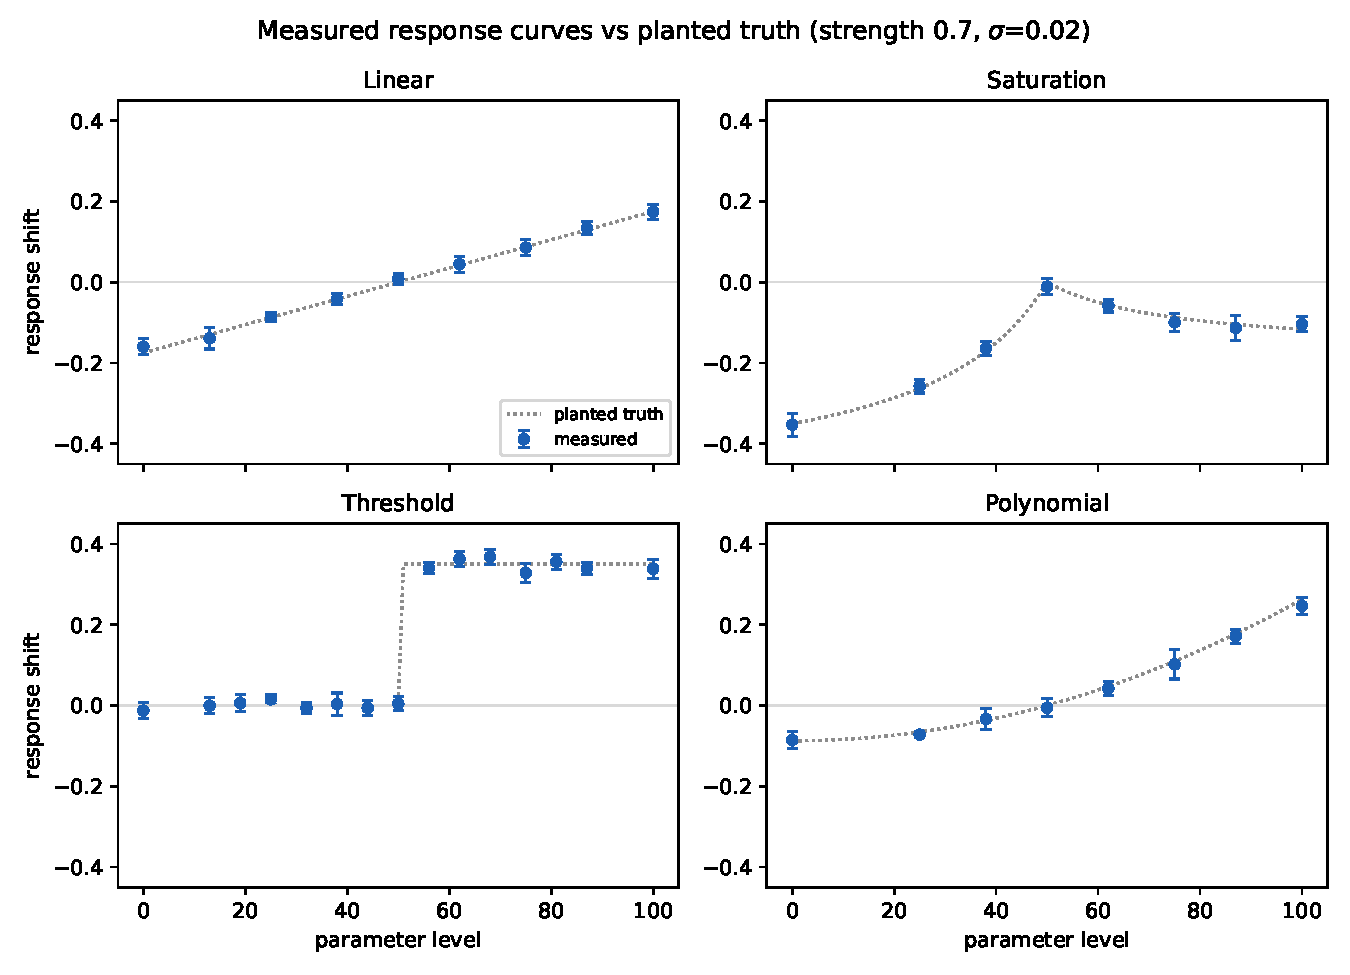
\includegraphics[width=\textwidth]{figures/fig1_shapes.pdf}
\caption{Measured response curves vs planted truth (dotted) at strength
0.7, $\sigma{=}0.02$. Points carry per-level error bars from local
noise (MAD).}
\label{fig:shapes}
\end{figure}

\subsection{The envelope}
\label{sec:envelope}

Figure~\ref{fig:envelope} assembles the worst-point deviations onto
the strength--noise plane. Every certified cell of the campaign sits
below $1.8\sigma$, most near or below one bar-width, with the $2\sigma$
certificate bound never approached. The map's edges are set by
coverage and budget --- where the walk declines to spend --- not by
accuracy loss: we find no condition inside the envelope at which a
measured point fell outside its own reported uncertainty.

\begin{figure}[h]
\centering
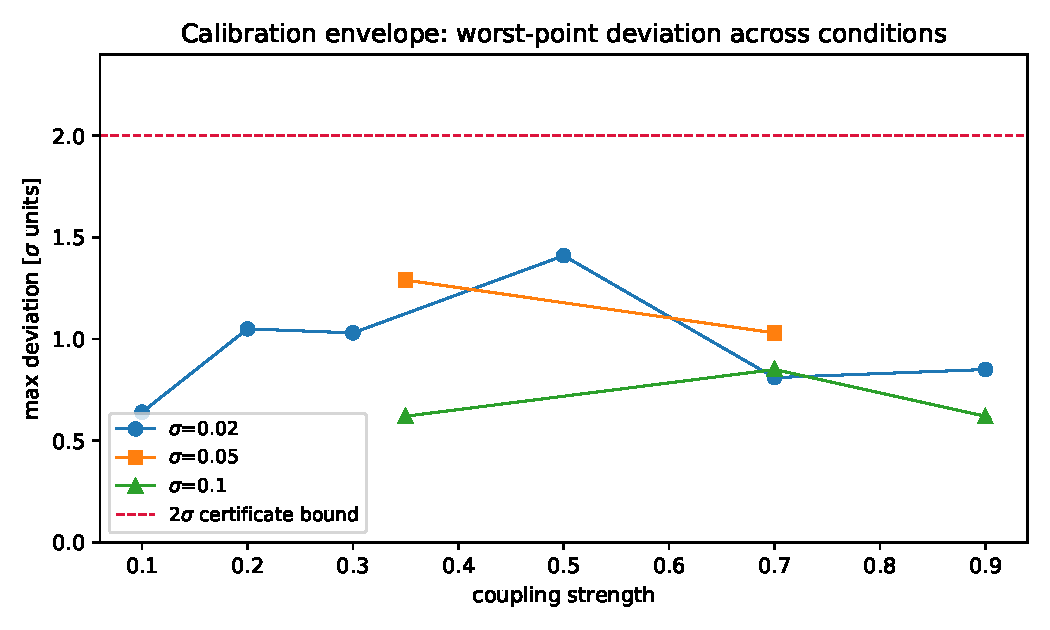
\includegraphics[width=0.85\textwidth]{figures/fig2_envelope.pdf}
\caption{Worst-point deviation across the strength--noise plane.}
\label{fig:envelope}
\end{figure}

\subsection{Walk economics: effort tracks signal}
\label{sec:cost}

Figure~\ref{fig:levels} shows levels walked against coupling
strength. The priced stop is the entire explanation, and it is
worth separating the two ways a measurement can spend effort,
because they answer different weaknesses. The walk can \emph{dwell
longer} at a level --- more trials, tighter bars, the classic
$\sqrt{N}$ averaging that turns noise down --- or it can
\emph{sample more levels}, resolving the curve's shape more
finely. Weak coupling calls for the first response, not the
second: a curve that spans only a few error bars has no shape
detail that additional levels could resolve, because any new point
would come back with a bar as tall as the feature one hoped to
see. Sampling level after level of a nearly flat, noise-dominated
region produces honest but uninformative points; the priced stop
declines to buy them. Strong coupling, conversely, makes shape
detail affordable: steep flanks keep gaps expensive, so refinement
pays, and the walk walks deeper. Under the campaign's uniform
per-run settings, wall time is comparable across strengths (the
runs of the weakest and strongest cells differ by minutes); what
scales with signal is the resolution purchased --- three levels at
strength $0.1$, nine at $0.9$ --- while per-level dwelling remains
fixed. The walk's own stop rule is thus its allocation model; a
full cost characterization (trials per level, dwelling versus
levels) was not recorded per level in this campaign and is left to
the follow-up.

\begin{figure}[h]
\centering
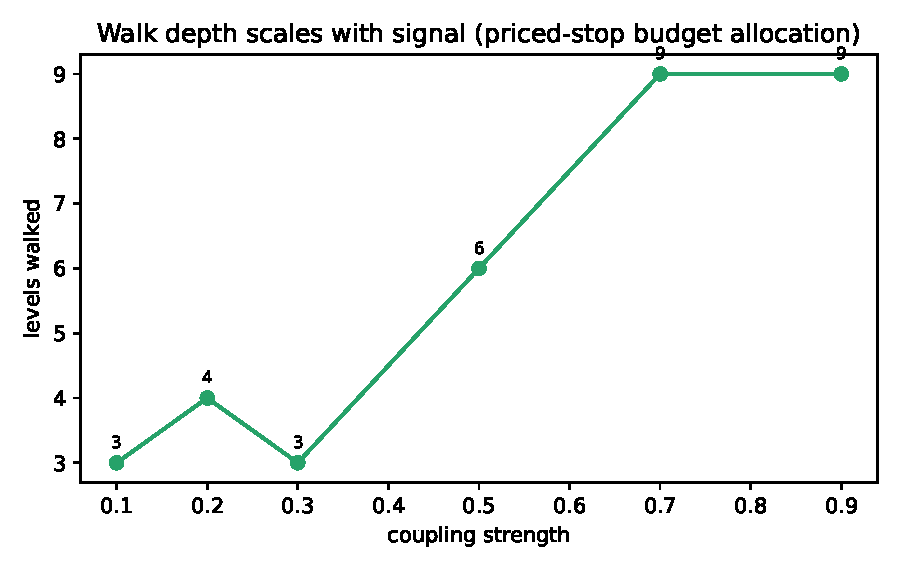
\includegraphics[width=0.7\textwidth]{figures/fig3_levels.pdf}
\caption{Levels walked vs coupling strength at $\sigma{=}0.02$.}
\label{fig:levels}
\end{figure}

\subsection{Non-stationarity}
\label{sec:nonstat}

Three regimes (Figure~\ref{fig:ns3}). Under \emph{noise that grows
through the run}, the curve stays certified while its bars fatten in
real time: late points carry roughly twice the uncertainty of early
ones, and the truth remains inside every bar. We state the size
plainly: the bars reach more than half the curve's amplitude ---
the measurement is certified but \emph{coarse}, and fine
characterization under that noise growth is not available at fixed
dwelling; it would require the longer-dwelling trade discussed in
\S\ref{sec:boundaries}. The walk's honesty is the result
here: it reports the degradation bar by bar rather than
certifying a precision the conditions do not support. Under
\emph{slowly drifting edge strength}, the walk captures structure
that tracks the moving edge: a deeper curve whose values follow the
coupling's journey rather than its start. Under \emph{fast drift},
finally, the walk does not converge --- correctly, for there is
nothing stationary to converge to: it probes to its budget's end
(twenty-two levels, the deepest walk of the campaign) and returns
an honest non-convergence rather than a fabricated average. The
boundary between measurable drift and unmeasurable drift is thus
drawn in data, by the walk's own refusal.

\begin{figure}[h]
\centering
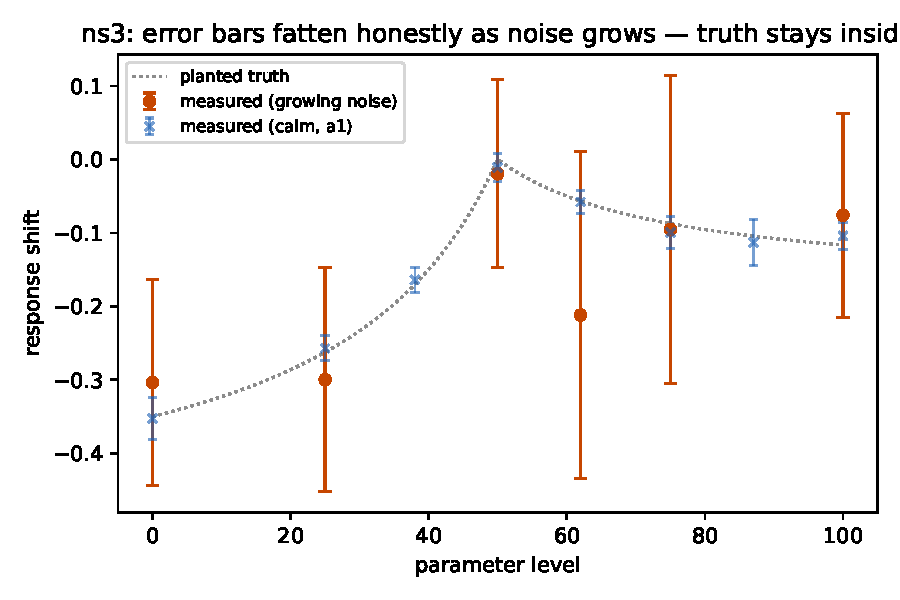
\includegraphics[width=0.75\textwidth]{figures/fig4_ns3.pdf}
\caption{Growing-noise cell: error bars fatten as conditions rot;
truth stays inside every one. Calm-cell bars (blue) for contrast.}
\label{fig:ns3}
\end{figure}

\subsection{Repeatability}
\label{sec:repeat}

The anchor cell (saturation, strength $0.7$) and both boundary
corners (floor $0.2$; wall $\sigma{=}0.10$) were repeated with a
second seed. All repeats certify within bars: the anchor pair agrees
at $0.69$ and $1.76\sigma$ worst-point, the floor corner at $1.05$
and $0.15\sigma$, the wall corner at $0.85$ and $1.07\sigma$. We
report the spreads as they are --- including the anchor's --- rather
than selecting the flattering member of each pair: repeatability of
the \emph{verdict} is the claim, and every verdict held.

\section{Measurement Honesty}
\label{sec:honesty}

An error bar says how repeatable a measurement is; it says
nothing about whether the measurement is attributed to the right
cause. A curve may be perfectly self-consistent and still be a
measurement of the wrong thing. The validity of the curves produced
here therefore rests not on the bars but on the planted sentinels
described in \S\ref{sec:design} --- and the discipline has teeth.
During the campaign's development, three defects in the measurement
chain were caught not by code review or unit tests but by exactly
these controls. First, \emph{frozen reads}: the bench answered
configuration queries with stored snapshots instead of recomputed
values, so a receiver that was holding perfectly still appeared to
report pre-push values --- the sentinels saw readings that no
motion could explain. Second, a \emph{warm-up race}: receivers kept
exploring inside their own warm-up phase while senders were already
probing, so early probe windows measured the receiver's own
initialization rather than the sender's push --- visible as
structure on parameters that carried no coupling. Third,
\emph{median poisoning}: the sender's own readings during its pause
blocks entered the receiver's observation window untagged, and the
scoring's time-based window could not tell them apart --- mixing
the two halved true amplitudes and manufactured apparent structure
on a dead parameter. Each fix was verified by the same sentinels
that exposed the defect. The lesson generalizes and we state it as
practice: honest bars are necessary, not sufficient --- each new
claim must re-validate its own measurement chain against planted
reality.

A second honesty rule concerns verdicts and badges. Runs fail for
reasons unrelated to the walk they contain: logging side-effects,
infrastructure expiry, queueing accidents. The campaign's scoring
therefore reads the walk's data directly --- the exported curve with
its per-point bars --- and classifies from the data, not from the
run's completion badge. Verdicts are disposable labels; the measurements beneath them
are what last; the evidence bundle retains the latter regardless of
the former. Every table and figure in this paper regenerates from
that bundle by a shipped script, and an independent recomputation
pass over all certified cells confirmed the reported numbers exactly.

\section{Boundaries}
\label{sec:boundaries}

We name the limits as measured, without softening.

\emph{Coupling physics.} The bench's edges are scalar and
additive-linear in the channel value; node-level nonlinearity is
where shape enters. Composition of measured curves through
intermediate nonlinearity is untested and is the subject of the
successor question; the bridge cells (diamond, chain, bidirectional)
are banked as data for it, not scored here.

\emph{Quiet bench.} Receivers hold by protocol throughout. No cell
measures against a receiver that resists --- an agent actively
optimizing during probe windows. That regime is untested.

\emph{Substrate class.} All evidence is from a mathematical bench
with closed-form planted truth. No physical substrate, no
production system, no live agent swarm appears in this certificate.

\emph{Multi-sender coverage.} With three or more concurrent walkers,
lease contention proved unfair in our structural cells: one sender
dominated the probe windows while others starved. Curves that were
taken remain valid --- at two walkers, coverage was complete and
both directions certified --- but full multi-sender maps await a
fairness mechanism in the coordination layer.

\emph{Initialization transient.} A receiver's first hold block
moves its parameters from their initial values to the hold point;
if a sender's walk is in flight, that motion is recorded as
structure on the sender's curves. The artifact is identifiable
(flat-then-jump shape on unplanted paths) and was reconciled in
every affected cell of this campaign; its definitive fix ---
seeding parameters at the hold point --- is straightforward and owed
before the successor work.

\emph{Adaptive dwelling.} The walk dwells a fixed number of trials
per level and \emph{reports} the resulting bar; it does not lengthen
measurement where bars are too fat to resolve further refinement.
Thin-bar acquisition through longer dwelling (a $\sqrt{N}$
configuration trade) was not swept in this campaign, and adaptive
or intent-directed dwell variants are unbuilt --- the latter
belonging to the steering question. Weak-signal curves therefore
retire at few levels rather than being re-measured to thinner bars
in place.

\section{Discussion}
\label{sec:discussion}

\paragraph{What a certified curve is the basis for.}
The certificate's clauses are ends in themselves for diagnosis ---
knowing the shape of a hidden influence is operationally useful ---
but their larger consequence is what becomes computable downstream.
Composition along graph paths requires response functions, not
boolean arrows: multi-hop prediction, and inversion of the map
toward a chosen operating point, are calculations over exactly the
objects this paper certifies. The successor question --- whether
measured curves compose through nonlinear intermediate structure ---
is the natural next gate, and the structural cells banked here
(diamond, chain, bidirectional) are its opening data.

\paragraph{From search to computation.}
Once a coupling map is measured, the search for good operating
points need not be blind: the optimum can be computed from the map,
and the agents' role narrows to exploring beyond the measured
envelope. A natural follow-up, not demonstrated here: an agent's
search runs, probing with attribution, could bank certified partial maps
as a by-product, so that search effort accumulates into
transferable structure knowledge rather than evaporating with the
run.

\paragraph{Future work.}
The measured boundaries are the work queue. Nearest term: lease
fairness in the coordination layer (multi-sender coverage at three
or more walkers), seeding parameters at the hold point (removing
the initialization transient at its source), and the
dwelling-versus-levels trade (thin-bar acquisition for weak and
degrading signals, including its adaptive variant). Beyond the
calibration scope: composition of measured curves through nonlinear
intermediate structure --- for which the structural cells retained
here are opening data --- and characterization against receivers
that resist, the step from a quiet bench toward live substrates at
large.

\paragraph{A measurement layer for shared substrates.}
The condition this procedure addresses --- multiple autonomous
actors perturbing a common substrate whose interactions are
invisible in their logs --- is increasingly the default in
agent-operated infrastructure. What such systems lack is not
telemetry but attribution: not ``the metric moved'' but ``this
actor's change moved it, by this much, with this confidence.'' The
calibrated curve is that object. The sentinels-only specificity
result matters most here: a method that occasionally invented
edges would be worse than none.

\paragraph{Relation to experimental design.}
The walk's sampling rule is close kin to classical response-surface
methodology~\cite{box1951rsm} and to modern model-based design of
experiments~\cite{jones1998ego}: sample where uncertainty or
disagreement is highest. The differences are the contributions:
those frameworks assume a single experimenter who owns the function
and can pause the world; the walk operates inside a live substrate
among other actors, attributes every reading through protocol
rather than experimental isolation, and prices its own stopping in
measurement units rather than a budget line. System
identification~\cite{ljung1999sid} remains the mature neighbor for
the quiet single-owner case; passive
methods~\cite{sugihara2012ccm} cannot see through self-generated
exploration noise at realistic budgets, as the detection study
already established~\cite{p1}. To our knowledge, no existing approach combines all three:
autonomous experimenters, a live shared substrate, and a certified
quantitative output.

\paragraph{One law worth naming.}
Measurement depth scales with evidence spent. The walk certifies at
coupling $0.1$ with three levels and at $\sigma{=}0.10$ noise with
fat bars because every level buys many trials and the bars are
earned; block-step detection, spending one contrast, stops earlier
on the same axes. The trade is not specific to this method: it
is the statistics of evidence, made operational by a stop rule that
turns the dial by itself. We expect the same law wherever
autonomous measurement budgets are priced against remaining
ignorance --- and the certificate's envelope is where that dial has
been measured for this class of substrate.

\bibliographystyle{plain}
\bibliography{references}

\end{document}
